\glsreset{clf}\glsreset{cbf}
This chapter ought to lay the basics of all shared control theory applied in the following chapters dealing with the design of a safe controller.

Based on \citep{bib:artstein}, who founded \glspl{clf} as described in \autoref{eq:lyap}, a \gls{cbf} can be created \citep{bib:org_control} from where the definition below is stated:
\begin{exa}[Control Barrier Function]
Given a system $\dot{x}=f(x)+g(x)u$, a \gls{cbf} exists if the below constraints are fulfilled:
\begin{subequations}\label{eq:reqs}
\begin{flalign}
x\in \mathcal{X}_u \hspace{0.3cm} &\Rightarrow \hspace{0.3cm} B(x) > 0  \label{req1} \\
L_gB(x) = 0 \hspace{0.3cm} &\Rightarrow \hspace{0.3cm} L_fB(x) < 0 \label{req2} \\
\{ x \in \mathcal{X} | B(x) \leq 0 \} &\neq \emptyset \label{req3}
\end{flalign}
\end{subequations}
\vspace{-0.6cm}
\begin{tabular}{r l l} 
where  & & \\
$B(x)$ & is a control barrier function & [$\cdot$] \\ 
$L_fB(x)$ & is the Lie derivative of $B(x)$ along the vector field  $f(x)$, i.e. $\frac{\partial B(x)}{\partial x}f(x)$ & [$\cdot$] \\ 
$L_gB(x)$ & is the Lie derivative of $B(x)$ along the vector field  $g(x)$, i.e. $\frac{\partial B(x)}{\partial x}g(x)$ & [$\cdot$] 
\end{tabular}
\vspace*{0.2cm}
\end{exa}
Note how \autoref{eq:reqs} put forth demands for the open loop system in oppose to \autoref{eq:barrier_constraints} that describes the closed loop system. \Autoref{req1} states essentially the same as \autoref{cer2}, i.e. when $B(x)>0$ the region is unsafe. This makes it possible to design both the unsafe region and the safe region. \Autoref{req2} put forth the requirement that the gradient along the vector field $f(x)$ must point away from the unsafe area bounded by the barrier zero-line whenever the input can not be controlled (except for the critical point as the system is in its equilibrium at this point). \Autoref{req3} simply states that the safe area must contain some states as control otherwise is impossible.
%
\section{The Control Law}\label{eq:control_for_safety}
It is convenient to divide the control law into two controllers. A controller that is used in an area close to the unsafe region and a controller used in the safe region. The reason for this divided control law is the ability to apply linear control theory in the safe area  (the system can be well approximated as a linear second order system, see \autoref{sec:model_slide}) and thereby offer all the benefits from linear control.

 %he old Chinese proverb, \textit{"Do not use a cannon to kill a mosquito"}, thus why not use a simple controller in the safe region

Defining the safe space excluding a small transition space between the safe and non-safe region as $\mathcal{Y}$ and the transition space as $\mathcal{T}$, a divided control law can be introduced as:
\begin{flalign*}
u(x) =
\begin{cases}
	\tilde{u}(x) \kk &\text{if} \mm x \in \,\, \text{\gls{Yfancy}} \\
	 k_0(x)  \kk &\text{if} \mm x \in \,\, \text{\gls{Tfancy}}
\end{cases}
\end{flalign*}
Thus the controller used in $x \in \mathcal{Y}$ will be referenced as a non-safe controller and the controller used in $x \in \mathcal{T}$ will be referenced as a safety controller or a controller ensuring safety. If the system is linerar, the non-safety controller can be determined by linear state feedback:
\begin{flalign}
\tilde{u}(x) = \bar{N}\,x_\text{ref} - K\,x
\label{eq:utilde}
\end{flalign}
\vspace{-0.8cm}
\begin{longtable}{p{.9\textwidth} p{.1\textwidth} p{.1\textwidth}} 
Where  & & \\
$K \in \mathbb{R}^{m \times n}$ is a constant feedback matrix with $n$ states and $m$ inputs & [$\cdot$] \\
$\bar{N} \in \mathbb{R}^{m}$ is a constant to ensure unity gain from reference to output & [$\cdot$] \\
$x_\text{ref} \in \mathbb{R}^m$ is the position reference& [$\cdot$]  \\
$x \in \mathbb{R}^{n}$ is the state vector& [$\cdot$] 
\end{longtable}
\vspace*{-0.2cm}
The two controllers can be combined as a linear combination determined by a parameter \gls{sigma} \citep{bib:org_control}. This ensures that the switch between the two controllers occurs with less fluctuations. 
\begin{flalign}
u(x,\tilde{u}) &= \sigma(x)k_0(x)+(1-\sigma(x))\tilde{u}(x) \nonumber \\
 &= \sigma(x)k_0(x)+(1-\sigma(x))(\bar{N} \cdot x_\text{ref}-Kx) \label{eq:control_law}
\end{flalign}
\vspace{-0.8cm}
\begin{longtable}{p{.9\textwidth} p{.1\textwidth} p{.1\textwidth}} 
Where  & & \\
%$u(x) \in \mathbb{R}^{m \times 1} $is a control signal where safety is ensured  & [$\cdot$] \\
%$\tilde{u}(x) \in \mathbb{R}^{m \times 1}$ is a control signal to the linear state space system such that $\tilde{u}=\bar{N}\cdot x_\text{ref}-Kx $ & [$\cdot$] \\ 
$k_0(x) \in \mathbb{R}$ is a control law that guarantees safety & [$\cdot$] \\ 
$\sigma(x) \in \mathbb{R}$ such that $0 \leq \sigma(x) \leq 1$ is a parameter that founds a linear combination between the two controllers & [$\cdot$] 
%$K \in \mathbb{R}^{m \times n}$ is a constant feedback matrix where $n$ is the number of states & [$\cdot$] \\
%$\bar{N} \in \mathbb{R}^{m \times 1}$ is a constant to ensure unity gain from reference to output & [$\cdot$] \\
%$x \in \mathbb{R}^{n \times 1}$ is the state vector& [$\cdot$] 
\end{longtable}
\vspace*{-0.2cm}
Note the two extremeties of  $\sigma(x)$:
\begin{flalign*}
\sigma(x) = 
\begin{cases}
0 \mm &\Rightarrow \mm \text{Pure control by pole placement, i.e. $u(x) = \tilde{u}(x) =  \bar{N}\cdot x_\text{ref}-Kx$ } \\
1 \mm &\Rightarrow \mm \text{Pure control for safety i.e. $u(x) = k_0(x)$ }
\end{cases}
\end{flalign*}
The interval between 0 and 1 can be refined such that the transition between the two control laws is not instantaneous. This smoothing can be performed with a continuous approximation of the unit step (a bump function) of $B(x)$ by introducing a scalar $\epsilon>0$ \citep{bib:org_control}:
\begin{flalign}
\sigma(x) = 
\begin{cases}
0 & \text{if} \mm B(x) \leq -\epsilon \\
-2  \left( \dfrac{B(x)}{\epsilon} \right)^3 - 3\left( \dfrac{B(x)}{\epsilon} \right)^2 +1 \kk &\text{if} \mm B(x) \in (-\epsilon,0) \\
1  &\text{if} \mm B(x) \geq 0
\end{cases}
\label{eq:smoothness}
\end{flalign} 
%
%
% 
A block diagram is depicted in \autoref{fig:controlsystem}.
\begin{figure}[h]\hspace*{-1.2cm}
	%\center
		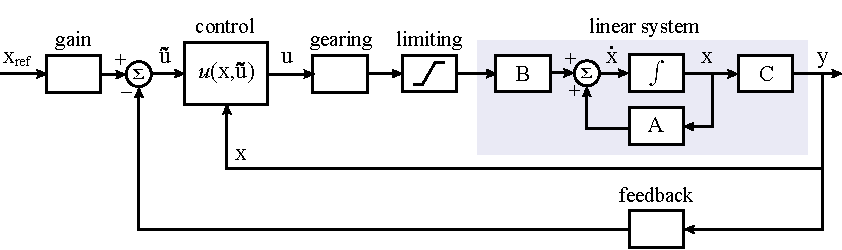
\includegraphics[scale=1]{control_system.pdf}
	\caption{Block diagram of the control system. The limiter limits the control signal such that it does not exceed the physical boundaries of the Da Vinci robot. The gearing ensures that there is a 1:1 mapping between the control signal and the physical position, i.e. meters for prismatic joints and radians for revolute joints.}
	\label{fig:controlsystem}
\end{figure}
\subsection*{Uniform Construction of $k_0$}
The control law ensuring safety can be found as \citep{bib:org_control}:
\begin{flalign}
k_0(x) = \begin{cases}
-\dfrac{L_fB(x)+ \sqrt{(L_fB(x))^2 + \kappa^2L_gB(x)(L_gB(x))^T}}{L_gB(x)(L_gB(x))^T}(L_gB(x))^T &\text{if} \mm L_gB(x) \neq 0 \\
0  &\text{if} \mm L_gB(x) = 0
\end{cases}
\label{eq:control_law}
\end{flalign}
Where $\kappa$ is a design variable. High values of $\kappa$ implies increased aggressiveness. \Autoref{eq:control_law} indeed ensures safety for the closed loop system $\dot{x} = f(x)+g(x)k_0(x)$. This is easily proven as:
\begin{flalign*}
L_{f_{cl}}B(x) = L_fB(x) + L_gB(x)k_0(x)
\end{flalign*}
For $L_gB(x) \neq 0:$
\begin{flalign*}
L_{f_{cl}}B(x) &= L_fB(x) + L_gB(x) \left( -\dfrac{L_fB(x)+ \sqrt{(L_fB(x))^2 + \kappa^2L_gB(x)(L_gB(x))^T}}{L_gB(x)(L_gB(x))^T}(L_gB(x))^T \right)  \\
&= L_fB(x) - L_gB(x)(L_gB(x))^T \dfrac{L_fB(x) + \sqrt{(L_fB(x))^2 + \kappa^2L_gB(x)(L_gB(x))^T}}{L_gB(x)(L_gB(x))^T}   \\ 
&= L_fB(x) - L_fB(x) - \sqrt{(L_fB(x))^2 + \kappa^2L_gB(x)(L_gB(x))^T} \\
&= - \sqrt{(L_fB(x))^2 + \kappa^2 L_gB(x)(L_gB(x))^T} \mm \leq 0 \mm \forall \mm x
\end{flalign*}
As all terms within the square root are squared, no imaginary numbers occur, as a result $L_{f_{cl}}B(x) \leq 0$ 

According to \autoref{eq:control_law}, when $L_gB(x) = 0$:
\begin{flalign*}
L_{f_{cl}}B(x) = L_fB(x) + L_gB(x)\cdot 0 = L_fB(x)
\end{flalign*}
As $L_fB(x)$ is constructed such that $L_gB(x) = 0 \hspace{0.15cm} \Rightarrow \hspace{0.15cm} L_fB(x) < 0 $ it is verified that $Lf_{cl}B(x)\leq 0 \,\,\forall x \in\mathcal{X}$. 

Thus the theory presented in this chapter allows a way to construct a controller such that safety is guaranteed if the constraints are obeyed. It may, however, be noted that when the controller is transferred to a digital system, the certificate is built upon an infinite sampling rate as the certificates are described in continuous time. Adopting the certificate to a discrete system is indeed a challenge worth respecting. 

The theory presented in this chapter shall in \autoref{chap:cbf_1d_static} be used to design a controller that ensures safety for slide movement and thereby illustrate the usefulness of the theory. It shall also be used in \autoref{chap:cbf_1d_dynamic} to establish the basics for surgery on a beating hearth.